\documentclass[conference]{IEEEtran}

\usepackage[british]{babel}
\usepackage{cite}
\usepackage{graphicx}
\usepackage{paralist}
\usepackage[hyphens]{url}
\usepackage{amsmath}
%\usepackage[pdftex]{hyperref}


\begin{document}
\bstctlcite{IEEEexample:BSTcontrol}

% paper title
% can use linebreaks \\ within to get better formatting as desired
\title{The Environmental Impacts of ICT Use:\\A User-Oriented Perspective}


% author names and affiliations
\author{
    \IEEEauthorblockN{Peter Cooper\IEEEauthorrefmark{1},
      Tom Crick\IEEEauthorrefmark{2}, Theo Tryfonas\IEEEauthorrefmark{1} and George Oikonomou\IEEEauthorrefmark{1}}
    \IEEEauthorblockA{\IEEEauthorrefmark{1}Faculty of Engineering,
      University of Bristol, UK
    \\\{peter.cooper,theo.tryfonas,g.oikonomou\}@bristol.ac.uk}
    \IEEEauthorblockA{\IEEEauthorrefmark{2}Department of Computing,
      Cardiff Metropolitan University, UK
    \\tcrick@cardiffmet.ac.uk}
}

% conference papers do not typically use \thanks and this command
% is locked out in conference mode. If really needed, such as for
% the acknowledgment of grants, issue a \IEEEoverridecommandlockouts
% after \documentclass


% use for special paper notices
%\IEEEspecialpapernotice{(Invited Paper)}


% make the title area
\maketitle


\begin{abstract}
In this paper we apply a whole-life assessment approach to estimate the
environmental impact of the use of ICT of an individual within the UK
over a one-year period. By estimating the energy and data consumption
of an average user's use of a typical device, and estimating
the associated energy usage (and thus CO$_2$ produced) of each stage
in the data chain, we are able to calculate the summed CO$_2$ value
for embodied carbon of an average device. 
% To enable this, market
% segmentation is undertaken to determine the average user and average
% use, along with market research to determine the average
% device. Analysis of device performance in difference behaviours is
% also undertaken.
Overall, device energy is seen to dominate; within device, desktops
dominate, both due to their high energy use for a given task, but also
their high standby power, which is the most significant point of
behaviour-driven waste. Geographical, behavioural and chronological
factors are all evaluated to be highly significant to the impact of a
user's ICT use, along with a number of secondary factors. Finally, we
present policy recommendations to further the understanding of the
factors affecting the environmental impact of ICT, particularly
focusing on sustainability, resource efficiency and the social
implications of ICT in a low-carbon transformation.
\end{abstract}

% For peer review papers, you can put extra information on the cover
% page as needed:
% \ifCLASSOPTIONpeerreview
% \begin{center} \bfseries
% \end{center}
% \fi
%
% For peerreview papers, this IEEEtran command inserts a page break and
% creates the second title. It will be ignored for other modes.
%\IEEEpeerreviewmaketitle

\begin{IEEEkeywords}
Life Cycle Assessment, Environmental Impact, Low Carbon Society,
Green ICT, Emissions, Policy
\end{IEEEkeywords}


\section{Introduction}

The creation, development and uptake of Information and Communication
Technology (ICT) is frequently cited as one of the most defining
characteristics of humanity over the last 100 years. Arguably, no
other development can claim to have had such a profound effect since
the first exploitation of fossil fuels. Today, no other service or
utility has as vast reach across the global population; over five
billion people now own an ICT device of some
kind~\cite{arup-et-al:2011}, more than those who have access to clean
water or sanitation. Despite this penetration, ICT use still continues
to grow; 90\% of all digital data generated has been created in the
last two years~\cite{bbcnews:2012}.

% ICT has demonstrated a continued
% exponential increase in processing power since the creation of the
% first computers in the 19th century. Today, a single Intel Haswell
% microprocessor contains more than 1 billion transistors in a
% three-dimensional configuration using a 22nm process, many orders of
% magnitude more processing power than all the computers involved
% landing the first humans on the Moon in 1969.  While the death of
% Moore's law has been long mooted, there is little evidence to suggest
% this growth will slow in the immediate future.

Further to the technical impact, there has been significant
socio-cultural impact. Relevant developments such as social
networking have redefined how individuals interact with one another;
digitisation of finance networks now permits the trading of incredible
(and increasingly abstract) wealth across the world over fibre and
microwave networks; and the computational power of modern
supercomputers has enabled us to better understand the makeup of
ourselves and our universe.

For all the benefits of ICT, it is also possible to identify negative,
unintended consequences -- political, social, economic and
environmental -- both now and potentially in the future. We also have
seen emerging UK imperatives around technology education and digital
skills~\cite{brown-et-al-toce2014}, the focus on (and profiling of)
online behaviour~\cite{oatley+crick:2014} alongside the global
priorities around cyber security~\cite{carr+crick-csss2015}, as well
as the explosion in technologies surrounding the development of smart
cities~\cite{cosgrave-et-al:2014} and future transport
infrastructure~\cite{cooper-et-al-sose}, all at some level predicated
on cost-effective and sustainable ICT infrastructure. Such costs beg
the question: just how sustainable is ICT? A complex question,
transcending short-term policymaking and infrastructural investments,
underpinning both global competitiveness and national security; the
consequences and our reaction to them will be one of the defining
challenges of the 21st century.

Rising concerns over man-made climate change and resource use, set
amongst a context of rapid user growth, has driven increased focus on
sustainability and the wider environmental impact of ICT. They have
been associated with 1.3\% of the world's total carbon footprint and
3.9\% of global energy use~\cite{plepys:2002}. While modest in terms
of overall impact, the continued penetration of ICT brings potential
concerns to how this will grow~\cite{yi+thomas:2007}. Like any product
or service, ICT has tangible environmental impacts across all parts of
its life cycle, from design to its disposal. However, our globally
interconnected but geographically dispersed ICT systems often make
assessment of the impact of a given ICT action complex and highly open
to interpretation~\cite{andrae+andersen:2010}. A process life cycle
carbon assessment
(LCA)~\cite{baumann+tillman:2004,iso14040:2006,bsi2050:2011} is a
common way of holistically exploring a product's life -- from cradle
to grave -- and logically identifying and categorising the
environmental impacts involved~\cite{malmodin-et-al:2014}; for
example, mobile phones~\cite{frey-et-al:2008,fehske:2011} and the
wider telecommunications industry~\cite{scharnhorst:2008}.
% \footnote{\url{http://www.greenbiz.com/blog/2011/03/08/exploring-ways-reduce-its-environmental-impacts}}

\subsection{Definitions}

\subsubsection{ICT}

In this paper we define the ``use of ICT'' as the use of information and
communication technologies that satisfies two criteria:

\begin{compactitem}
\item Uses stored-program architecture, excluding a myriad of other
  electronic devices in use, as well as older forms of information
  technology (books, etc);
\item Primary function is that of the creation, processing or display
  of data; excluding electronic devices that use stored-program
  architecture only as a supplement to a different core function, such
  as cars, white goods, electrical toothbrushes, watches and bike
  computers.
\end{compactitem}

We propose that the majority of ICT meeting these two criteria can be
summarised as follows:

\begin{compactenum}
\item Smartphones: A mobile phone based upon a stored-program
  architecture with a range of communication technologies (e.g. GSM, GPS,
  Bluetooth, etc.).
\item Tablets: A device that is possible to be held in one's hand but
  has no GSM connectivity.
\item Laptops: A device that weighs less than 4kg but greater
  than 1kg, and has the ability to run off batteries for a
  tangible duration.
\item Desktops: A device that has no ability to run off batteries for
  a tangible duration, with a primary function to service
  user requests, rather than those of another computer.
\item LAN: The primary channel between devices and Internet-supporting
  infrastructure Ethernet, WiFi, 3/4G).
\item WAN: The supporting infrastructure of the Internet linking
  servers and nodes.
\item Servers: The destination for data transferred from the device
  (also referred to as data centers).
\end{compactenum}

Items 1 to 4 are classified as `Devices'. These are items that are
created for their own purpose to serve the user, not to service the
existence of other ICT items. Items 5 to 7 are classified as
`supporting infrastructure'. These are items whose primary function is
to service the existence of the devices.

\subsubsection{Individuals}

The user is defined as an individual in the domestic, private, or
public sectors; this excludes any industrial setting. Industry is
deemed to have extreme variation in the characteristics of ICT use,
and the integration of ICT and mechanical/chemical systems make valid
identification and categorisation problematic. For example, a worker
in an aluminium refinery may operate a computer embedded in an
electrolysis machine with a total power consumption of over 1MW; how
much of this can be accredited to ICT could involve extensive analysis
of pre- and post-ICT states of all dependent/related industries. As
such, workers in industry will simply be modelled as standard private
sector workers with an average amount of ICT in their occupation.  We
will consider specific types of user/non-users individually, as well
as an aggregated `average' UK citizen. We will also include the impact
of non-users and nearly-non-users. The specific user types and how
they make up the UK market will be discussed a later section.

\subsubsection{Environment Impact}

We consider environmental impact exclusively as greenhouse gas (GHG) emissions using the CO$_2$e metric~\cite{bsi2050:2011,ieaco2em:2014}. This encompasses global warming potential of CO$_2$ as well as the relative global warming
severity of other greenhouse gases, relative to the severity of
CO$_2$. 

% As discussed, other elements of environmental impact will be
% presented and discussed in our conclusions and recommendations.

\subsubsection{Life Cycle Stages}

The life cycle stages of the devices are outlined below:

\begin{compactitem}
\item {\emph{Creation}} -- Conception to Gate: the design, extraction of raw
  materials, manufacture and all actions necessary to retail and
  deliver the device to the user.
\item {\emph{Use}} -- Gate to End Use: from the users first ownership
  of the device to when it ceases to be their property. Broken down
  into two subcategories:
\begin{compactitem}
\item Use -- Device: the actions of the device itself.
\item Use -- Supporting Infrastructure: made up of supporting ICT and
  other supporting infrastructure.
\end{compactitem}
\item {\emph{End of Life}} -- End Use to Grave: from when the device
  ceases to be property of the owner, to when all components have been
  reused/recycled/disposed.
\end{compactitem}


% \section{Literature Review}

% There are a number of existing studies in the area of environmental
% impacts of ICT, and specifically the energy and GHG impacts associated
% with devices and services; this review identifies what are perceived
% to be areas of strong and weak focus in recent domain research, and
% uses this appreciation to determine areas of novel and valuable work.

% %\subsection{Areas of Strong Focus}

% \subsection{GHG Emissions Associated with Manufacture}

% By looking at the latest information on the level and growth of CO$_2$
% emissions, it is possible to decompose into key driving
% factors~\cite{ieaco2em:2014}. Existing research has explored the
% relationship between the mass of the device and the embodied GHGs
% associated with the manufacture
% stage~\cite{williams:2004,teehan-et-al:2010}. Protocols have also been
% developed to provide guidance for estimating the emission reductions
% that could result from the provision or sourcing of low or zero carbon
% ICT services~\cite{steenhof-et-al:2012}.

% \subsection{Environmental Impact of Disposal}

% The energy associated with disposal is negligible relative to the use
% and manufacturing phase~\cite{williams:2004}. Technology manufacturers
% such as Apple publish
% data\footnote{\url{https://www.apple.com/environment/reports/}}
% relating to environmental impact for each of their products, motivated
% by customer pressure on the embodied carbon of their purchases. Their
% environmental data for products shows this as a relatively
% insignificant stage: typically accounting for 2-4\% of the GHG
% emissions associated with a device, with production and use phase
% typically the greatest contributors. While consequential environmental
% impacts of disposal are significant, direct GHG emission is not.

% \subsection{Impact of Cloud Computing}

% Recent research has focused on the potential reductions in GHG
% production through a shift to cloud
% computing~\cite{williams-et-al:2014}, and the rebound effect of
% digital data becoming cheaper and easier to consume meaning more and
% more is used is well documented. There is a strong commercial
% motivation for such users, with the potential to save high-intensity
% ICT organisations substantial savings from switching to the cloud.

% %\subsection{Areas of Weak Focus}

% \subsection{Chronological Variation of GHG Emissions of Electricity Supply}

% While the Realtimecarbon
% project\footnote{\url{http://realtimecarbon.org/}} was launched in
% 2009, no analysis of the impact of user behaviour on this has been
% conducted: the domain literature almost exclusively refers to average
% figures for GHG impact of electricity from the national grid. This is
% widely considered to be acceptable practice, although little
% justification of this has been carried out. From our
% observations\footnote{\url{http://ukedc.rl.ac.uk/ext_stats_uk.html}},
% the carbon output of the UK National Grid can vary as much as +/-24\%
% from the standard value quoted by the Carbon
% Trust\footnote{\url{http://www.carbontrust.com/}} of 445.48g
% CO$_2$e/kWh in a short period of time, potentially giving significant
% inaccuracy in existing analyses.

% \subsection{Geographical variation of GHG emissions of electricity supply}

% The environmental impact of ICT use in different countries,
% particularly the variation in the electrical generation carbon, is
% poorly explored in existing literature. Outside of developing
% countries, the environmental sustainability of ICT is a low priority
% issue. However, even within developed countries, little research has
% been undertaken as to how changes in national grid generation policy
% affects the sustainability of ICT, although the modelling of other
% countries provides some insight into this~\cite{malmodin-et-al:2014}.

% \subsubsection{Device interchangeability}

% Little research appears to have been undertaken on the extent to which
% the rise of tablet and smart phone ownership has reduced the use of
% laptops and desktops, though anecdotal evidence claims both
% substantial positive and negative
% impacts~\cite{andrae+andersen:2010}. There is little financial
% motivation for manufacturers to suggest that customers `downsize'
% their ICT use to smaller devices as it would be motivating the sale of
% lower priced devices. If however, the device power is a dominant part
% of power use, downsizing could be a viable method of power
% reduction~\cite{frey-et-al:2008}.

% \subsubsection{Accurate User Behaviour Data}

% Limited literature exists that analyses the relative importance of
% different uses of ICT. As part of this, the power consumption of
% individual components, and how these vary based on the type of use, is
% also very limited. Regulatory groups such as Energy
% Star\footnote{\url{https://www.energystar.gov/}} estimate a total
% electrical annual consumption (TEC), based on an average device power
% multiplied by an average hours per day of use; there are also
% international datasets available from the US Energy Information
% Administration\footnote{\url{http://www.eia.gov/cfapps/ipdbproject/}}.
% Primary research in this area is ultimately constrained by cost; by
% observation it is clear that ICT is used in a number of ways, each
% having significant effect on the device's power use.


\section{Scope}
% added some context from removed literature review -- REFS??
We have identified four principle areas -- user behaviour,
chronological variation, geographical variation and device
interchangeability -- that are the principle focus of our LCA design,
model and primary data tool. These have been through existing gaps in
the domain literature around the GHG emissions associated with
manufacture, the environmental impact of disposal, the wider impact of
cloud computing and the chronological and geographical variation of
GHG emissions of electricity supply.

Geographical and chronological variations are easily applied to the
existing system. This allows modelling of the carbon cost of
electricity generation. Behavioural and device substitution themes can
be addressed through a strong focus on the use-device and
use-supporting infrastructure life cycle stages. Creation will be
included in the LCA though end of life will not. This is because the
latter is perceived to have negligible impact on energy and GHG
emissions, whereas the contribution by the former is deemed
significant and will provide a comparison with the use phase
impacts. The GHG and energy of each prototypical day for each user
type (exclusive of embodied) will be displayed chronologically across
the day. The final values of annual GHG and energy will be displayed
in two breakdowns: by user group contribution and by life cycle stage
for each user.

\subsection{User-Centric Input}

To accurately capture user behaviour, it is necessary to capture it
from primary data at the source. While this is time-consuming, it is
beneficial to design a tool that is capable of direct user input. This is not
only for future development of the LCA, but also to influence the
design process to carefully consider the real life nuances of user
behaviour.

This tool works on the concept of prototypical days. These are defined
as days that usually have very similar patterns. For example, all days
where the user is at work and in the office on a typical work
schedule. We expect that 90\% of a user's days can be categorised with
2-4 prototypical days, and that the rest can be acceptably amalgamated
into the rest. The tool permits the user to enter what each of their
devices is doing, to a half hour resolution over the 24 hour duration
of a prototypical day. This includes inputting when the device is on
but not actually in use.  The option to select a different country
demonstrates the significance of geographical variability.

\subsection{Upscaled Use}

Finally, the individual is asked how many of each prototypical day
makes up a year, with the request that all sum to 365 days. The values
given for each device for each prototypical day can then be multiplied
by the number of such prototypical days in a year, and then summed, to
evaluate the individuals' overall impact in a year.

\subsection{Energy Calculation}

Energy is calculated in half hour sections through the prototypical
day. Energy per section is calculated by summing the Device, LAN, WAN
and Server energy values. Device energy is found as described above,
while the remaining elements are calculated based upon the data
throughput (D) and a number of constants (all energy values are in
Joules, and the energy-data constants are given in J/MB):
\begin{align*}
E_{LAN} &= E_{standby} + k_{energy}-data_{LAN} * D)\\
E_{WAN} &= k_{energy}-data_{WAN} * D\\
E_{server} &= k_{energy}-data_{server} * D
\end{align*}

\subsection{Carbon Calculation}

Carbon produced is calculated as a function of energy consumed in each
section, geographical location and time. The latter two data sets are
discussed later in this document, and take the form of look- up
tables. The carbon produced is calculated as below (CO$_2$ produced is
measured in g, and time-location constants are given in g/J,
translated from the g/kWh that is input):

\begin{align*}
C_{device} &= k_{C\_time\_location} * E_{device}\\
C_{LAN} &= k_{C\_time\_location} * E_{LAN}\\
C_{WAN} &= k_{C\_time\_location} * E_{WAN}\\
C_{server} &= k_{C\_time\_location} * E_{server}
\end{align*}

\section{Data Collection Strategy}

%^\subsection{State of Market}

The purpose of this section is to determine the average device within
each device type: Phone, Tablet, Laptop and Desktop.

% \begin{compactdesc}
% \item[Phone:] In the UK, the mobile phone market is dominated by four key players,
% with Apple and Android taking the majority market
% share\footnote{\url{http://media.ofcom.org.uk/facts/}}. A logical
% approach would be to transpose a sales by phone model metric, over a
% five year period, to a given companies market share, to roughly
% estimate the phones of that player in the UK. We can observe some of
% the most popular phones in use today, but not all, and further more
% these do not cover a significant share of all usage as there are many
% models available in this mature market.

% \item[Tablet:] In recent years, the tablet market, has developed
%   significantly, with significant R\&D and new product lines from the
%   major manufacturers, periodically releasing updated models. 
% As a result, the tablet market can be estimated by
% device ownership with much greater ease.

% \item[Laptop:] The laptop market is a highly saturated and mature market, even more
% so than the mobile market. A vast number of different manufacturers,
% each with large number of models, makes this market impossible to
% segment into distinct key players, let alone into individual devices. 
% Instead the typical device characteristics are estimated from previous
% research, benchmark resources and EnergyStar data, as is frequently
% the case in previous research.

% \item[Desktop:] The desktop market is similar to the laptop market, though perhaps
% even more mature and saturated. Not only does a vast array of
% manufacturers exist, but a great deal of re-branding exists, with
% retailers reselling devices that manufacturer’s retail
% themselves. Again, this market is impossible to segment into distinct
% key players, let alone individual devices. And as above, the typical
% device is estimated from previous research, benchmark resources and
% EnergyStar data, as is frequently the case in previous research.
% \end{compactdesc}

\subsection{Manufacture}

%\subsubsection{Embodied GHG}

This paper does not have a strong focus on the embodied energy and
carbon of ICT devices resulting from the production phase in the life
cycle; instead the key focus is the use phase. However, not taking the
energy and carbon involved in producing the devices that individuals
use would not give a satisfactory answer for the environmental impact
of an individual's ICT use in one year. Furthermore, any conclusions
about changes in the use phase need points of comparison.

As such, this paper does not focus on the
embodied carbon and energy of devices, but does take it into account
in the analysis of an individual's ICT use. Using relevant
research which has had a strong focus on embodied energy and carbon,
an analysis was undertaken to give reasonable estimates for typical
embodied GHG in each device type. These are then used to identify a
value for the footprint of an owner of each device type by estimating
the device lifetime. Finally, due to the disparity in the estimated
values for Apple products and those of other manufacturers, an average
value was achieved by drawing on the market share of Apple products
for each device type; the resulting figures for each device type
are: Desktop: 127.275 kgCO$_2$e; Laptop: 85.456 kgCO$_2$e; Tablet:
45.9 kgCO$_2$e; Phone: 18 kgCO$_2$e.

\subsection{User Input Strategy}

The purpose of this section is to determine the average user of ICT
devices; using primary market research we have produced a high-level
market segmentation of all ICT users. For each segment we have defined
key behavioural points and the device types owned by each; the
resulting market segmentation can be seen in
Figure~\ref{fig:itusersuk}, with our estimations of the relative
proportions of each segment can be seen in
Figure~\ref{fig:marketshare}.  Using primary market research into user
behaviour, we decided upon the types of days of use; typically
`average weekend' and `average weekday' for most users. For each day a
timetable of use, to a resolution of 0.5 hour slots, was specified.

\begin{figure*}
\centering
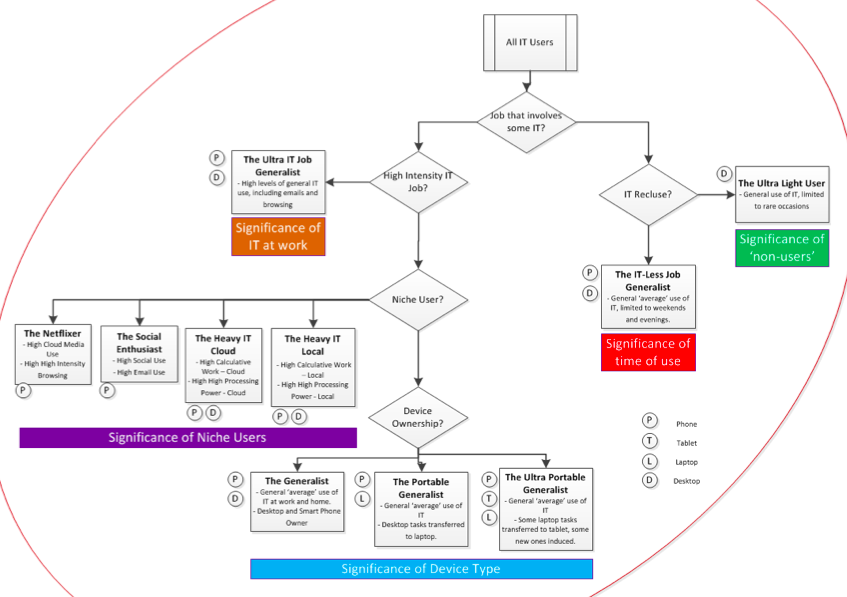
\includegraphics[width=0.8\textwidth]{images/ukitusers_ownership_signif.png}
\caption{ICT Users in UK, device ownership and significance to this analysis}
\label{fig:itusersuk} 
\end{figure*}

\begin{figure}
\centering
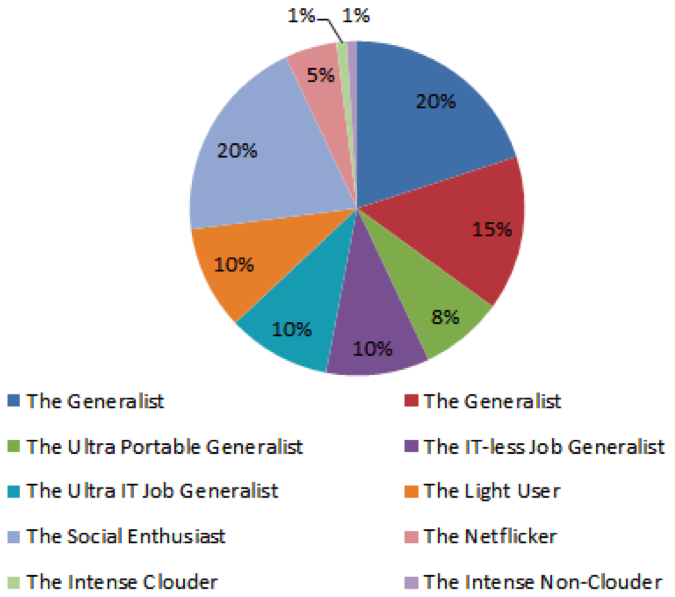
\includegraphics[width=0.9\columnwidth]{images/ukitusers_marketshare.png}
\caption{Assumed market share of ICT user types in UK}
\label{fig:marketshare} 
\end{figure}


\subsection{Device Use}

We wish to define an average user's ICT use and to explore how a
device behaves in general under different use cases.  A device can be
used for many different purposes, any one of which we will define as a
use case.  To identify a suitable selection of use cases, we initially
identified a large number of possible use cases, which were then
filtered to satisfy the following criteria:

\noindent {\textbf{Excluding those that show unusual behaviour in the
device components:}} this excluded gaming, where Graphics Card power
can be up to 250\% of a standard desktop’s power, discussed in the
other components section later.

\noindent {\textbf{Including those that are most prevalent:}} this
excluded listening to music and scanning.

\noindent {\textbf{Excluding those that are insufficiently different
to an idle state:}} this excluded background system tasks such as
watchdogs and network updates.

\noindent {\textbf{Including those that are necessarily distinct in
order to comment on the key issues within our scope:}} including cloud
and non-cloud variations of similar tasks.

For this analysis we categorise the power consuming components of
a device into four categories:

\begin{compactitem}
\item CPU: Including all integral elements.
\item Display: Inclusive of the power used by the display only.
\item Network Components: Any power-consuming component that is used to transfer data in or out of the device.
\item Other: Inclusive of all power-consuming components
  of the device not covered in the previous categories as well as
  peripherals. Includes RAM, hard drive, motherboard, graphics
  card, sound cards in the first element; printers, scanners and input
  devices in the second.
\end{compactitem}

A use case has four principle characteristics:

\begin{compactitem}
\item CPU Power Factor: the variation of the CPU’s power in a given use case.
\item Display Power Factor: the variation of the Display’s power in a given use case.
\item Other Power Factor: the variation of others in a given use case.
\item Data Flow: the magnitude of data (summation of in and out) flow during a use case.
\end{compactitem}

The aforementioned power factors affect the given power use of each
device component, on average, in a given use state. These are
calculated thus:
\begin{align*}
CPU &= CPU idle power * CPU power factor\\
Display &= Display average * Display power factor\\
Other &= CPU idle power * Other power factor
\end{align*}

CPU power use and CPU utilisation does not follow a linear
relation. In practice, the CPU consumes tangible power when idle, and
then increases from this to anything from 2-10 times the idle power at
100\% utilisation. During primary research, we observe that certain
types of use case manifest themselves as different tasks on different
devices. For example, high intensity browsing, such as viewing of a
video on YouTube~\cite{schien-et-al:2013} will typically be done at a
resolution of the device or lower. As such, the task will require less
processing power on smaller devices. Others will not scale in this
way, for example a word document will be the same size and complexity
of word document regardless of device size.

We theorise that for scalable tasks, the downscaling of task
intensity can be approximated as balancing out with the decrease in
processing power for smaller devices. For non-scalable tasks, we
theorise that applying the same approximation will be of
little inaccuracy, as such unscalable tasks are typically of such low
processing intensity that the practical utilisation will be only
slightly higher on less powerful CPUs.  These assumptions culminate in
having a `power factor' for a given use case that is common to all
four device types.

As such CPU power use varies with undertaken task intensity.
Through primary research we have identified that
instantaneous CPU power use, on modern CPUs, is typically low --
$<$30\% for most tasks -- and that average CPU intensity lower
still. Through primary research we have obtained estimations of
average CPU powers for all of the use cases defined; these can be seen
in Figure~\ref{fig:cpuintensity}. We can see that the majority of
applications use little power above idle, with a few select tasks
actually using the full power of the device. This aligns with other
research in the field of CPU design and use. For a standby mode of any
device, the CPU rests at its idle power.

\begin{figure}[!ht]
\centering
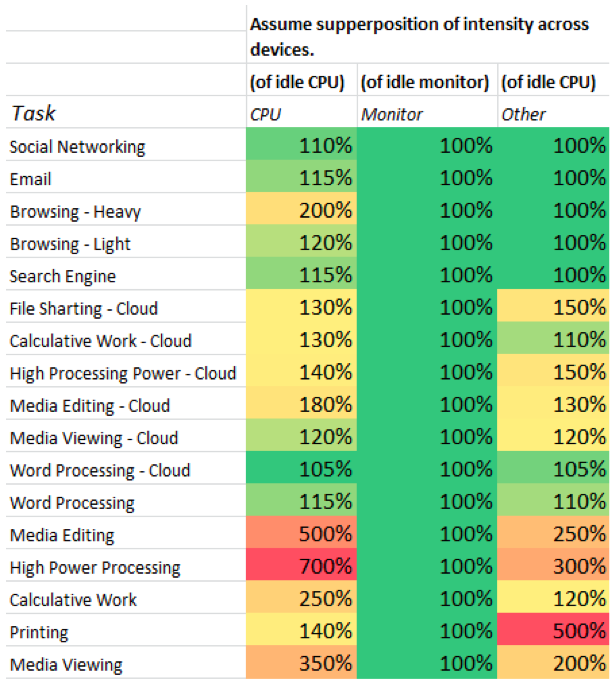
\includegraphics[width=0.9\columnwidth]{images/cpuintensity_usecase.png}
\caption{CPU intensity by use case}
\label{fig:cpuintensity} 
\end{figure}

Research suggests display power is not dependent upon the level of
activity on a screen: changing content does use energy in the
display. Research also suggests that in modern displays, the exact
colour of the content is not related to power consumption. The only
distinct characteristic proven to influence the power consumption is
the brightness setting of the display~\cite{malmodin-et-al:2014}. This
is typically unrelated to a task; indeed, it could be said that
individuals may lower the brightness during long working hours, such
as extensive typing, or raise it when the quality and clarity of the
image is crucial, such as when watching a film. This however, is most
probably a matter of personal taste, and the
inter-use-case-brightness-level variation is likely to be less
significant than the individual’s average preferences on brightness.

Network connection power is typically perfectly inelastic to data, and
as such is evaluated as constant for each type, discussed by device in
later sections. As such, no power factors exist for network
devices. The power from the remaining components is difficult to
estimate without considering the power uses of individual devices. As
such, these can be inferred from the remaining observed power use of a
given device when network and CPU powers have been taken out, as
determined in later sections. With regards to power factors, there are
two elements that exist:

\begin{compactitem}
\item The use of peripherals to service a task: the inclusion of extra
devices to facilitate an end, such as printers, scanners and such. The
power impact of such devices is given by their independent power
ratings.

\item The power of internal components in relation to task intensity:
  research suggests most other components scale very little with task
intensity, and change their power more based on specific nuances - for
example the HD with file sharing, the graphics card with media
viewing. As such, this is considered to be a smaller influence than
the peripherals
\end{compactitem}

% For each task, the other power factor will be estimated based on the
% above factors. The other power factor will then be multiplied by the
% device’s idle CPU power. With the assumption of equal intensity, while
% this will hold true for B, it will also result in some inaccuracies in
% A, implying the peripherals will scale with the device’s CPU. In
% mitigation, some of these situations will never be observed, such as
% printing from a phone. Others will, such as printing from a laptop,
% but we will note these inaccuracies, which we deem to be small, as a
% point of further improvement.


% \subsubsection{Use -- Supporting Infrastructure}

% The energy associated with data flow which is consumed by supporting
% infrastructure is outlined in more detail in supporting information
% section 4, and summarised in Table 7 below.

The final data requirement for this analysis is the carbon intensity
of the energy used by the individual and their ICT-related
activities. As previously mentioned, this project assesses the
chronological impact of the ICT use, and this has been achieved using
primary data collected from the Realtimecarbon project, rather than a
static average value for the GHG impact of grid electricity.

The figure commonly quoted for UK National Grid carbon intensity is
445.48g CO$_2$ (via Carbon Trust) per unit of energy (1kWh), however
in reality this figure changes over the course of the day, and over a
longer time period, depending on what energy sources are being used
and their relative contributions to the current grid mix.


\section{Results}

\subsection{Chronological View}

Figure~\ref{fig:generalist_weekday} demonstrates the energy use, by
the device that causes it, and then by component, for The Generalist’s
`Average Weekday'. Point A shows the minuscule standby power
(erroneously including the screen being on) of the phone
overnight. Point B highlights the increase in device power of
printing. Point C demonstrates the only perceptible time the phone’s
energy consumption is tangible, during heavy browsing. Point D
demonstrates the deactivation of the work computer as the user travels
home; Point E shows the activation of the home desktop upon arrival,
entering standby mode. Point F shows the increase in device power due
to a small period of media viewing; shortly before this we see the
only tangible power consumption of WAN and Servers, during the high
data task of Heavy Browsing. Immediately, we can observe that in
almost all situations, the phone’s power is imperceptibly small
compared to the desktop power. Secondly, we can observe that idle
computer power is a significant point of wastage.

\begin{figure}[!htp]
\centering
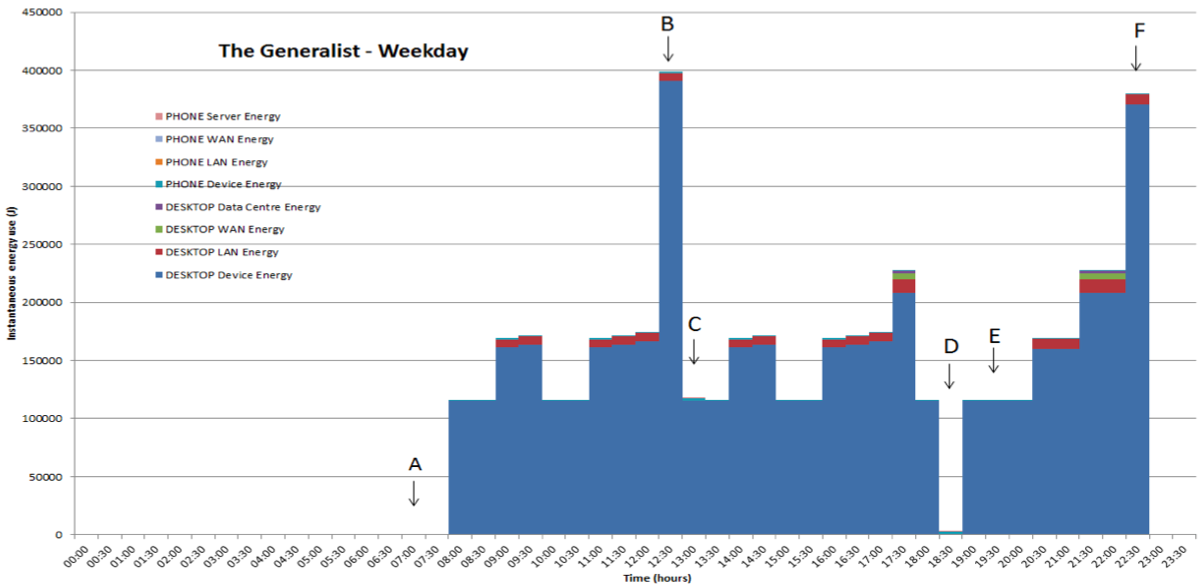
\includegraphics[width=0.9\columnwidth]{images/generalist_weekday.png}
\caption{Energy use by device and component}
\label{fig:generalist_weekday} 
\end{figure}

\subsection{By User}

Figure~\ref{fig:energyuse_co2e_overyearbyuser} demonstrates the
energy, in use CO$_2$e and embodied CO$_2$e by user type.
Observe the substantial variation in the environmental
impact across user types; we will discuss the significance of this
in the conclusion.

\begin{figure}[!htp]
\centering
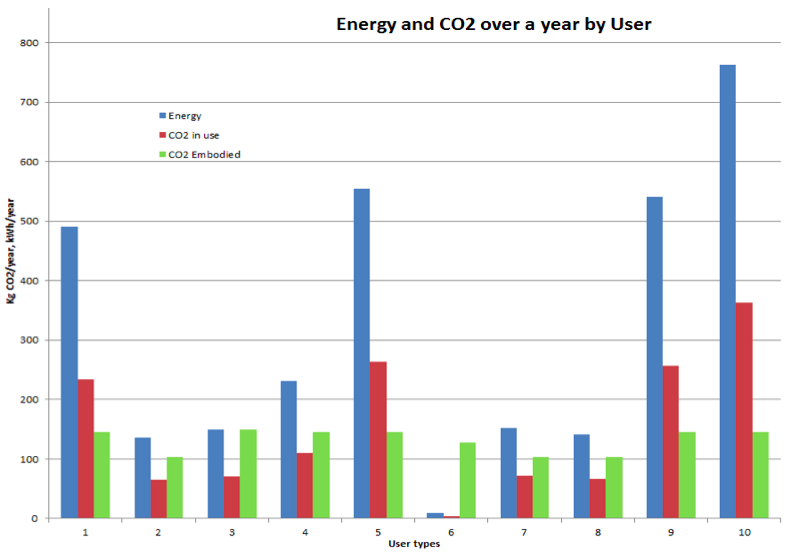
\includegraphics[width=0.9\columnwidth]{images/energyuse_co2e_overyearbyuser.png}
\caption{Comparison of energy use and CO$_2$e for users}
\label{fig:energyuse_co2e_overyearbyuser} 
\end{figure}

\subsection{By Infrastructure}

Figure~\ref{fig:energyusecomparison} demonstrates the energy use by
infrastructure type. Immediately we can observe that the device
dominates the power use across all user types covered. LAN appears an
order of magnitude smaller, WAN and Server an order of magnitude
smaller again, and roughly equal to each other. We also observe that
the exact proportions of all four energy types vary considerably
depending on the user type.

\begin{figure}[!htp]
\centering
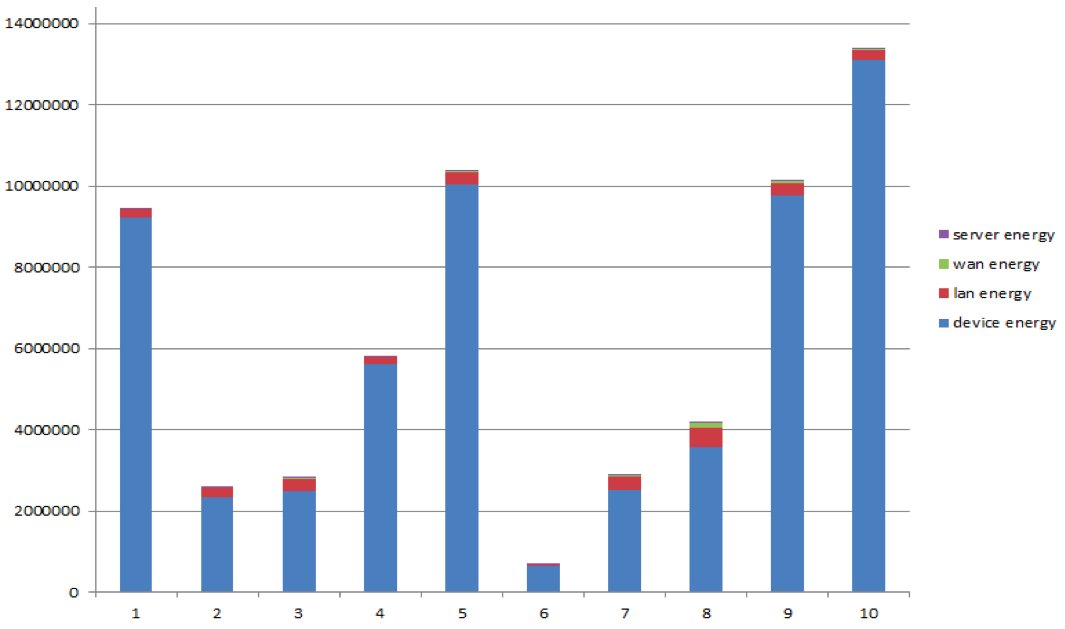
\includegraphics[width=0.9\columnwidth]{images/energyuse_comparison.png}
\caption{Comparison of energy use of device and infrastructure}
\label{fig:energyusecomparison} 
\end{figure}

% \subsection{Estimation of ICT Impact of an Average UK Individual in
%   One Year}

Final calculations show that, when prototypical days and user type
distribution is taken into account, the impact of one average UK
individual in one year is:

\begin{compactdesc}
\item[Total energy use:] 259kWh
\item[Total in use carbon:] 123.7kg
\item[Total embodied carbon:] 127.1kg
\end{compactdesc}

% The tabulated values of energy and carbon by each prototypical day for
% each user, which have been used to produce this calculation, can be
% seen in supporting information section x?.

% \subsection{Validation}

% The approximate total annual energy consumption (kWh) for devices/user
% seem reasonable when compared to EnergyStar TEC and sust-it.net
% analysis. The latter states:

% - Desktop: approx 50kWh - 200kWh per year, \pounds 6-\pounds 28\\
% Laptop: approx 6kWh-55kWh, \pounds 1-\pounds 8\\

% Our equivalent cost of \pounds 39 seems a realistic value for the time
% period.  Our slightly higher value can be attributed to the inclusion
% of both wider infrastructure, standby power and the inclusion of
% extreme user groups such as The Intense Clouder and The Intense Non-
% Clouder.


\section{Conclusions}

% \subsection{Significance of Chronological Context}

% To further evaluate the significance of carbon variation we will
% compare two identical situations: the social enthusiast using social
% networking on a 3G phone at different times of the day.

% As Figure~\ref{fig:ghgimpact_times} shows, the grid carbon varies
% within a sufficient proportion of the day’s hours that users are
% active in both the highs and the lows. As such, social networking on
% the commute to work is about 6.7\% more carbon intensive than a
% session shortly before bed.

% \begin{figure}[!ht]
% \centering
% 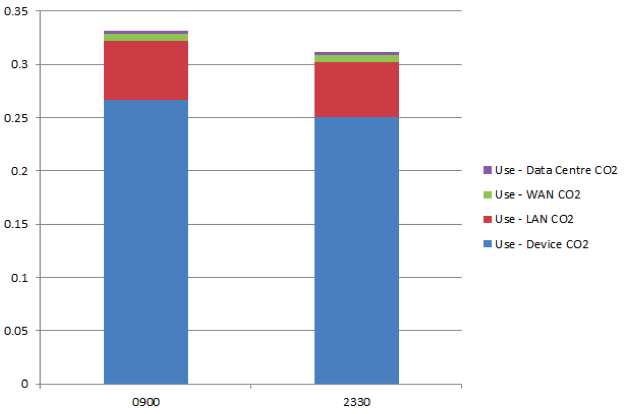
\includegraphics[width=\columnwidth]{images/ghgimpact_times.png}
% \caption{GHG Impact of Identical Action at Different Times}
% \label{fig:ghgimpact_times} 
% \end{figure}

\subsection{Significance of ICT at Work}

The benefit of exploring varying user behaviour is the ability to
differentiate domestic and professional ICT use. The Generalist, the
ICT-less Generalist and Ultra ICT Generalist all own the same
devices. The ICT-less Generalist only uses a desktop at home;
Generalists use it approximately 40\% of their working hours, the
Ultra ICT Generalist about 80\%.  This non-linear relationship can be
explained by the significance of standby power. Having a computer on
at work is the key factor -- this immediately adds a large base power
use (Generalist vs. ICT-Less Generalist), but further use of the
computer makes a much smaller difference (Generalist vs. Ultra ICT
Generalist). ICT-Less Job Generalist does a little more desktop use at
home as a result and delegates some of the would-be-desktop day time
activity down to a phone, but both are insignificant in
comparison. This highlights the significance of workplace policies to
minimise idle computer time. The energy use of workplace computers
left on overnight is not covered in our LCA and could be hugely
significant.

% The varying desktop energy use over a day can be seen in
% Figure~\ref{fig:ghgvariation_userworkrelatedit}.

% \begin{figure}[!ht]
% \centering
% 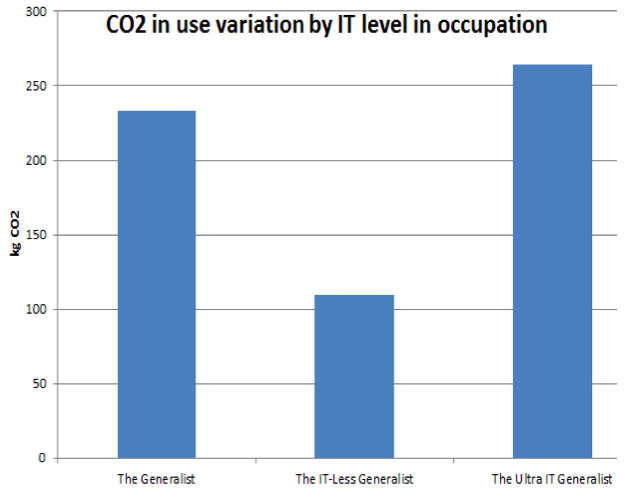
\includegraphics[width=0.9\columnwidth]{images/ghgvariation_userworkrelatedit.png}
% \caption{GHG variation with user work-related ICT}
% \label{fig:ghgvariation_userworkrelatedit} 
% \end{figure}

\subsection{Significance of Non-Users}

Figure~\ref{fig:energyusecomparison} shows that the in use CO$_2$ of
near-non users is an order of magnitude smaller than other users. This
is not only driven by low use, but exemplified by the efficiency of
which they use their desktop: by turning it off immediately after use,
they accrue no standby power wastage. However, even though they are
modelled to only own a desktop, the embodied carbon of it is highly
significant and as such they cannot be neglected as a user group --
their total carbon footprint is only 20\% lower than a Portable
Generalist. Furthermore, despite their efficiency of use, this
translates overall to a heavy impact per hours of use -- 1.36kg/hour
compared to 0.068kg/hour for The Portable Generalist.

\subsection{Significance of Varying Task Types}

Even though the overall impact is dominated by device energy,
situations exist that span many different proportional makeups. It is
important that these are considered should any of these situations
become particularly popular in the future. Furthermore, the analysis
of individual behaviour allows us to evaluate common perceptions of
the environmental impact of given device uses. Logic might suggest
that streaming a video (using large amounts of data and increasing CPU
load) would be poor behaviour environmentally. However, the Social
Enthusiast, who typically keeps his device on longer (particularly on
the weekends) to perform a relatively low intensity task is far
worse. Furthermore, the Netflicker could be considered to be using the
concept of cloud efficiency -- streamed videos are typically of a
lower codec complexity than downloaded or DVD/BluRay based
video~\cite{schien-et-al:2013}.

\begin{figure}
\centering
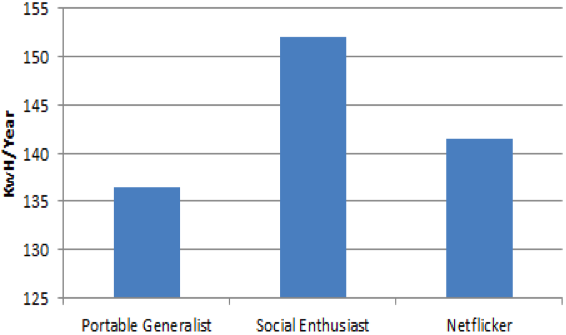
\includegraphics[width=0.9\columnwidth]{images/comparison_users_devices.png}
\caption{Comparison of notebook/phone use}
%\caption{Comparison of different users and their devices}
\label{fig:comparison_users_devices.png} 
\end{figure}

\subsection{Significance of Interchangeability of Devices}

Modelling similar behaviour across different devices provides the
ability to comment on how devices can be interchanged and the effects
of this. In our model we assume the Generalist and the Portable
Generalist have identical behaviours -- the increase in potability of
the device does not, for the prototypical days covered, induce
additional ICT demand. For the Ultra Portable Generalist, we model
there being a slight increase in ICT use induced by the inclusion of a
tablet. The tablet is on the individual almost as much as a phone is,
and this increase in portability is somewhat more significant than the
desktop-laptop transition. Some tasks are deemed to be down-scalable
to the tablet, but a lower percentage than those down-scaled the
previous situation. Furthermore, some tasks on the phone are scaled up
to the device, due to the overlap of possession.

% Device interchanging is a voluntary process that has come to light
% with the proliferation of different kinds of devices in the consumer
% market. Where there was once desktops and a few laptop models, there
% is now a myriad of desktop, laptop, tablet and phone devices, and a
% myriad of hybrids not covered in this report. In reality, device
% interchanging is not a simple process, and this was reflected in our
% user types.

% In reality, only a few exceptions to this can be perceived -
% using a laptop in meetings, taking a laptop to a friends house - but
% these are relatively infrequent events in the scale of an individuals
% life. Furthermore, the vast majority of tasks undertaken on a desktop
% can be undertaken on a laptop.

Although the energy step up from phone to tablet is much smaller than
the step down from laptop to tablet, the saving here roughly equates
to the sum of the actions scaled up from the phone and the induced
actions. When the greater embodied carbon is then included, we can see
the inclusion of new smaller device has actually resulted in a greater
environmental impact of the Ultra Portable Generalist than the
Portable Generalist. Crucially, this difference is small compared to
the differences between both of these users and the original,
desktop-based Generalist. It could be logically concluded the extra
carbon for The Ultra Portable Generalist is a small price to pay for
the extra benefits of a tablet, and certainly preferable to The
Generalist. Indeed, one could theorise that a policy to give away
tablets in return for old desktop computers would, at least in theory,
be highly effective.

% \subsection{Relative Significance of Device and Supporting
%   Infrastructure}

What is perhaps the strongest trend in all of our findings is that
device energy dominates. The logical progression of this is the CPU
intensity of a task is a far better indicator of its environmental
impact, at least in most situations, than the data flow. If accurate,
this suggests that efforts to reduce server and LAN power would be
better spent on reducing device energy. Ultimately this is an
incredibly complex topic involving wider socio-psychological and
market forces and is only briefly considered here. From the theory
here, an ideal solution appears to make 98\% of individuals use only a
phone; this is clearly an unacceptable suggestion. Crucially though,
the relationship between devices, behaviour and carbon is highly
significant and demands further research, providing huge potential for
national policy formulation~\cite{smart2020:2008,ruth:2011}.

\begin{figure}
\centering
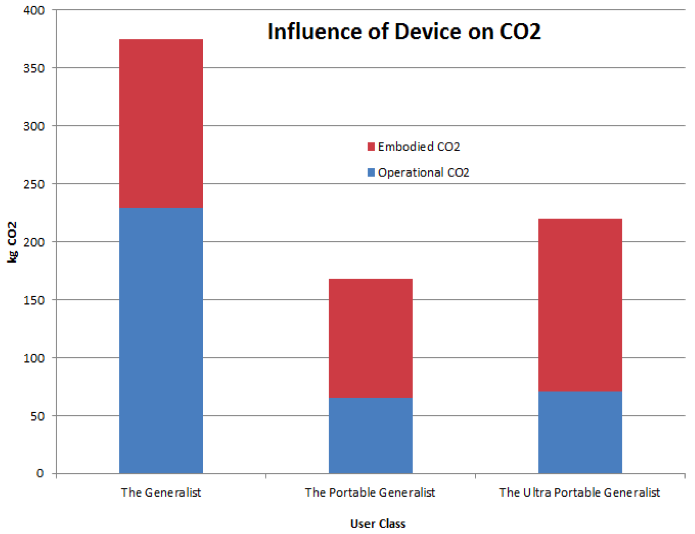
\includegraphics[width=0.9\columnwidth]{images/ghgimpact_devicetypes.png}
\caption{Variation in GHG impact for different device types}
\label{fig:ghgimpact_devicetype} 
\end{figure}

\section{Recommendations}

\subsection{Personal}

\subsubsection{Downscaling}

As the above results show, different use characteristics produce wide
variation in the consumed energy and CO$_2$ production. The most
apparent variation is in the contrast between desktop use and
smartphone use. This gives credence to recommendations to use a
smartphone over a desktop where possible, especially for low power
tasks such as internet browsing. This raises practical issues, so a
significant benefit can also be made by the transition from desktop to
laptop with much more ease. With the exception of the 2\% of Intense
Clouders and Intense Non-Clouders, the vast majority of users' tasks
should be able to transition flawlessly (at least in the technical
sense).
% Light users, whose embodied dominates their overall carbon impact,
% could make a substantial reduction by using a laptop over a
% desktop. Furthermore, these individuals could purchase a smart phone,
% even if for their own entertainment, and make negligible difference to
% their overall impact.
In a commercial context, the operating costs of an office run off
laptops as opposed to desktops would be significant, and also provide
more flexibility.

\subsubsection{Re-scheduling}

The results also shows a significant variation in the CO$_2$ produced
and the time of day it is produced. It could be suggested that users
carry out certain activities at particular times to make the most of
the CO$_2$ per energy constant at that time but in practice this may
not be suitable for the majority of users, and the benefits may not
out-weigh the inconvenience. However, if the highest device energy
users -- the Intense Clouders and Intense Non-Clouders -- have any
flexibility as to when they are able to undertake their high power
processing, careful monitoring of the live carbon value could result
in as much as a 45\% reduction in its carbon if done at a low point
rather than a high point. These user types also have the highest
proportion of device energy. That is to say, those with high energy
use over a year typically pay a larger share of that (on the
assumption WAN and Servers are not paid for by the user directly). As
such, if carbon-based taxing or demand-based pricing, as has been
suggested, becomes a reality, this time consideration will make
economic as well as environmental sense.

\subsection{Commercial}

%\subsubsection{No Standby}

As highlighted throughout, on a work day, considerable power is wasted
through idle desktops. Screen savers could be an easy quick win for
the effort setting them would, but are unlikely to reduce the overall
wastage by more than 30\%. Suggesting individuals turn off their
computers whenever they are not directly using them is likely to be
completely impractical in the workplace. However, turning them off
outside working hours could result in a substantial saving, albeit not
modelled here. Some pioneering companies operate network protocols
that attempt to shut down the computer, unless aborted by the user, at
the end of working hours. There is some synergy between this and the
downsizing recommendation. Laptops would not only use less power in
general, but waste far less sitting in idle.

\subsection{Policy}

\subsubsection{Carbon Grid Tax}

Clearly encouraging large users of electricity, as well as to a lesser
degree the average user, out of high-peak times is beneficial for
reducing the environmental impact of ICT, but also to the national
grid, to whom grid variation causes immense financial cost.

If energy providers are unwilling to switch to `smart pricing' --
demand-based electricity pricing -- then perhaps a
carbon tax, charged based on what CO$_2$ intensity the grid is at any
one point, will give an economic incentive for people to change
behaviour. Furthermore, this will both improve the environment, but
also reduce the cost of variability to the UK National Grid. This will
also make de-carbonisation easier (as low carbon generation is
typically baseload (geothermal, nuclear) or unpredictable (wind,
solar). Another consequential benefit would be the motivation of the
public for the government to reduce the carbon of the grid and so
reduce their carbon tax. As we have seen in the run up to the 2015 UK
elections, energy policy is an extremely politically-sensitive topic;
however, an aggressive national agenda for ICT-specific focus on
energy management, would -- if successful -- provide a potential model
for other sectors where reduced electricity use and lower carbon
footprint could be achieved~\cite{smart2020:2008,ruth:2011}.

\subsubsection{High-Power Leisure Device Regulations}

In the same way that car buyers are put off inefficient cars by road
tax, a tax on high power consuming computer components could be the
answer, such as 200W+ graphics cards. While this may be effective, it
would also be hard to enforce, and ethically questionable if other
more common commercial entertainment products (for example,
televisions) were not taxed similarly. Implying individuals should
adjust their leisure time to be more sustainable has become a
increasingly unpopular viewpoint. Labelling however, such as common
practice on other products sold in the EU, could be a reasonable
compromise, encouraging consumers to make the choice themselves. These
have been highly effective on fridges and other white goods.

% unless policy-related, remove due to lack of space

% \subsection{Further Work}

% This section will briefly summarise suggestions for model improvements
% discussed throughout:

% \begin{compactitem}
% \item Monitor brightness: inclusion of the input of the brightness level a user typically sets
% their display to will improve display accuracy across all devices, but
% specifically small devices.

% \item Specific devices within categories: as discussed throughout,
% inclusion of the option to input specific devices will further
% increase accuracy across all devices.

% \item Tool automation: to increase accuracy and ease of primary
% research, the tool could be translated into an executable program,
% which runs in the background, monitoring the task, data and energy
% flows. This could also reference live carbon resources at that
% instantaneous moment of action, allowing rapid collection of
% near-flawless data.

% \item Relationship between desktop cost and CPU idle power: an
% alternative method for estimating the idle power of a given desktop
% (to accommodate the large variation), may be to assume that the cost
% of a desktop (adjusted to today's value, where purchased
% historically), is proportional to the power of the CPU. Anecdotal
% evidence suggests this could be a valid relationship and individuals
% are more likely to know when they purchased their desktop, and for how
% much, than they are the CPU it contains.

% \item Chronological context of embodied carbon: if the dimension
% of time is important to use CO$_2$, it is logical to assume it influences
% the embodied carbon also. As such, it could be suggested that embodied
% carbon for a given device will depend upon the grid power used, the
% techniques used, the availability of raw materials and so on. As such,
% dependant upon when it was made. This will not only be a useful
% investigation to see how older and new devices compare on embodied
% carbon, but also to evaluate if the embodied carbon (per CO$_2$ of
% device) is general increasing or decreasing over time.
% \end{compactitem}


%\newpage

% trigger a \newpage just before the given reference
% number - used to balance the columns on the last page
% adjust value as needed - may need to be readjusted if
% the document is modified later
%\IEEEtriggeratref{28}
% The "triggered" command can be changed if desired:
%\IEEEtriggercmd{\enlargethispage{-5in}}

% references section
\bibliographystyle{IEEEtran}
\bibliography{gsict2015}

% that's all folks
\end{document}


